% CAISE'19 Conference - Paper on Ontological Analysis of the GRADE Taxonomy

% Using IOS template and predefined packages.
%\documentclass{IOS-Book-Article}

\documentclass[runningheads]{llncs}
%\documentclass[smallextended]{svjour3}       % onecolumn (second format)
\usepackage{mathptmx}
\def\hb{\hbox to 10.7 cm{}}

% Use unicode as document charset.
\usepackage[utf8]{inputenc}

% Symbols packages: to include many non-standard symbols.
\usepackage{amssymb}
\usepackage{eurosym}

% Amsmath package: includes \eqref to reference equations.
\usepackage{amsmath}

% Color control.
\usepackage[usenames,dvipsnames]{xcolor}

% Graphicx package: to include EPS figures in the document.
\usepackage{graphicx}

% Url package: to use the \url{} command to output URLs, which breaks them into two lines if needed.
\usepackage{url}

% Xspace package: to automatically place spaces when needed after macros.
\usepackage{xspace}

% Hyperref package: to handle crossreferencing commands to produce hypertext links in the document 
\usepackage{hyperref}

% Soul package: to use the \hl{} command to highlight text, useful to spot "to-do" items.
\usepackage{soulutf8}

\usepackage{float}

% Colorinlistoftodos package: to insert colored comments so authors can collaborate on the content.
\usepackage[colorinlistoftodos, textwidth=20mm, textsize=footnotesize]{todonotes}
\newcommand{\bruno}[1]{\todo[author=\textbf{Bruno},color=green!30,caption={},inline]{#1}}
\newcommand{\vitor}[1]{\todo[author=\textbf{Vítor},color=red!30,caption={},inline]{#1}}

% Macro definitions.
\newcommand{\awreq}{\textit{AwReq}\xspace}
\newcommand{\awreqs}{\textit{AwReqs}\xspace}
\newcommand{\evoreq}{\textit{EvoReq}\xspace}
\newcommand{\evoreqs}{\textit{EvoReqs}\xspace}
\newcommand{\zanshin}{\textit{Zanshin}\xspace}
\newcommand{\znn}{\textit{ZNN.com}\xspace}


% Begin the document.
\begin{document}

% Predefined cofiguration for the IOS template.
\pagestyle{headings}
\def\thepage{}

% The preamble begins here.
%\begin{frontmatter}   

% Title and date.
\title{Ontological Analysis of a Decision Making Taxonomy}
%\title{Towards a Ontological Analysis of the GRADE Taxonomy}
%\markboth{}{Somewhere 20XX\hb}

\author{Bruno Carneiro\inst{1} \and
	Bruno Duarte\inst{1} \and
	Renata Guizzardi\inst{1} \and
	Anna Perini\inst{2} \and \\
	Angelo Susi\inst{2} \and
	Vítor E. Silva Souza\inst{1}
}
\authorrunning{Carneiro et al.}

\institute{Ontology and Conceptual Modeling Research Group (NEMO),\\ Federal University of Espírito Santo, Brazil \and
Fondazione Bruno Kessler, Italy\\
\email{guimaraescarneiro@gmail.com, brunoborlini@gmail.com, rguizzardi@inf.ufes.br, perini@fbk.eu, susi@fbk.eu, vitorsouza@inf.ufes.br
}}

\maketitle
% Abstract.
\begin{abstract}
%Software Systems are getting increasingly complex, for a software to be considered commercial,  more requirements to be implemented and higher quality standards to be achieved.Because of that, the decision-making process is vital for any kind organization, decisions need to be made in strategical, tactical and even in operational levels. In order to provide support and improve the decision making process, the GRADE taxonomy was created. In this position paper, we provide an ontological analysis of The GRADE taxonomy with the Decision Making Ontology. We argue that with the ontological analysis we can help to improve the contribution of the taxonomy, by presenting a deep discussion about the relations that exists between the elements of The GRADE and that are not presented.
%Motivation
While software is becoming a pervasive element in our daily activities,  the engineering processes pertaining to its development, maintenance and evolution require flexible and effective decision-making. To support these processes, guiding its decision-making process, practical tools have been defined. The GRADE taxonomy is proposed for supporting decision-making about software systems architectures. It has been validated on decisions taken in several industrial projects, evidencing its effectiveness. 
%Problem
Nevertheless important weaknesses were pointed out by this validation, like the lack of clear relationships between elements of the decision-making taxonomy, which makes it difficult for a new user to learn how to use it correctly.

%Contribution
With the aim to address this limitation, we performed an ontological analysis of GRADE using a well-founded core ontology on decision-making. This allowed us to identify concepts that were implicit, besides supporting us in understanding the relationships between the concepts already composing the taxonomy.

%Paper
In this paper, we describe the ontological analysis of GRADE. Moreover, we illustrate the results of this analysis by applying the resulting model to guide a decision-making process for selecting the most appropriate software architecture/configuration for a release planning tool. 
We also discuss the limitations of the proposed ontological analysis, as well as some implications for future work.


\keywords{Decision-Making process; The GRADE Taxonomy, Decision-Making Ontology, UFO}

\end{abstract}

% Keywords.

%\end{frontmatter}
%\markboth{January 2016\hb}{January 2016\hb}

% Main contents of the paper, separated by section in different files.
%%% Section start %%%
\section{Introduction}
\label{sec-intro}
%
%Requirements prioritization is an important activity in the software life-cycle. During the development process, decisions about which ones are the most important requirements for a software system should be made. After that, during the operation of the system, decisions about how the software shall evolve and what path to take to guarantee the longevity of the software (now as a product) are as important as the ones made during design-time. Besides that, the quality of a software product is directly related to the ability of the software product satisfy the needs of the users by providing the desired features~\cite{sommerville2008engenharia}. Because of that, planning the development and also the evolution of a software, in order to specify the correct requirements and future updates are vital for the success of a software.As an example, we can mention World of Warcraft, the world's most successful massive multi-player online role playing game, had part of its success credited to the fact that the creators had over 12 years of updates and expansions precisely planned and prioritized. On the other side, bad decisions about the requirements implementation can lead to delays, cost extrapolation and in more serious cases, the failure of a software project~\cite{babar2011challenges}.
Software is becoming  pervasive in our daily activities,  from social activities, home management, to traveling and professional activities. On one side, as users we expect high quality software, on the other side,  as software producers, our main objective is to keep high  the quality of the software system we deliver, so to remain competitive in the market. This requires high quality development, maintenance and software evolution processes, which rest on continuous and effective decision-making to cope with technology changes and new  market's requests. 

%Software Systems are getting increasingly complex. 
For instance, for a software to be considered commercial, more requirements need to be implemented and higher quality standards need to be achieved. However, in most cases, because of limitations such as time and budget, not all functionalities can be implemented in the correct time, which contributes to the importance of well-grounded decisions about the path a software project should take during development. Besides, developing a software system is not an easy task on its own, since they usually are composed of many sub-systems, hardware components and even external software. Because of that, the decision-making process is vital for any kind of organization: decisions need to be made in strategical, tactical and even in operational levels of an organization~\cite{aurum2003fundamental}. Moreover, for organizations that deal with complex and time-consuming products, such as software systems or software-intensive products, this is specially true, since a bad decision can delay a project for months, extrapolate the cost budget and, in the most serious cases, cause the organization to go bankrupt. 

To cope with these problems, providing support and improving the decision making process, Papatheocharous et al.~\cite{papatheocharous2015decision,papatheocharous2018thegrade} propose the GRADE taxonomy, which intends to provide a structured instrument for collecting and documenting decision-making evidence. Its intent is to help software organizations in their projects. 

The GRADE taxonomy has been validated on decisions taken in several %29? 
industrial projects, providing evidences about its effectiveness. 
%Problem
%Nevertheless important weaknesses were pointed out by this validation, like the lack of  clear relationships between elements of the decision-making taxonomy, which makes it difficult for a new user 
%adopter of the taxonomy 
%to learn how to use it correctly.
%However, as a taxonomy, GRADE
For instance, the fact that this taxonomy provides a series of concepts (as categories) but does not specify the relations between theses categories, has been identified as a limitation, which can make it difficult for a new user to learn how to use it correctly.

As understanding the relationships between the concepts inherent to a domain are crucial part to understand the domain itself~\cite{guarino2015discussrelationship}, in this paper, we intend to fill this gap by providing an ontological analysis of the categories presented in the GRADE taxonomy, using the decision-making ontology, originally proposed in~\cite{guizzardi2018aligning}. Finally, it is important to mention that we chose the decision-making ontology to be the base of this ontological analysis because it is directly related to the domain of the taxonomy and because it is grounded in the Unified Foundational Ontology (UFO)~\cite{guizzardi:phdthesis05,guizzardi-et-al:ideas2008}. UFO is a widely accepted foundational ontology, providing a complete set of domain-independent concepts and their relations, that can be successfully used to provide an ontological interpretation and domain clarification.
%Because of these factors, plus the fact that a decision making process is a difficult task on its own that many researchers and international standards such as the IEEE Recommended practice for software requirements specifications~\cite{ieee830-1998} and the CMMI~\cite{team2010cmmi} take requirements prioritization as an important management activity for any organization.

%As Ruhe~\citeonline{ruhe2005decision} pointed out, requirements prioritization is known to be difficult because of the uncertainty and overall incompleteness of the information available. Moreover, there is a number of different techniques and frameworks presented in the scientific literature and even in international standards for requirements prioritization, each one with its own specificities, strength and weakness. Some methods are based on international standards while others are presented in the scientific literature and tested over years through case study, however, to the best of our knowledge no proposal takes into consideration the use of reference ontologies to support the decision making during the requirements prioritization process.

%This paper presents an work in progress of an ontological analysis of two requirements prioritization techniques presented in the scientific literature based on the decision making ontology~\cite{guizzardi2018aligning}


The rest of the paper is organized as follows, Section~\ref{sec-background} presents the GRADE taxonomy and the ontological foundations underlying the decision-making ontology. Section~\ref{sec-ontology} presents the ontological analysis of the GRADE taxonomy made based on the decision-making ontology. Section~\ref{sec-example} presents an illustrative example and a discussion about the added value of using the ontology. Section~\ref{sec-relatedwork} lists previous works about using ontology in Decision Making and ontological analysis of other decision-making methods. Section~\ref{sec-discussion} proposes a discussion 
%threat to validity and 
on the implication of this work and, finally, Section~\ref{sec-conclusions} concludes the paper.



%%% Section start %%%
\section{Background}
\label{sec-background}
%Background  (1 p.): a) GRADE b) UFO +BDT?


\subsection{The Grade Taxonomy}
\label{subsec-taxonomy}

The GRADE taxonomy~\cite{papatheocharous2015decision,papatheocharous2018thegrade} was proposed as a tool to support the organization and characterization of the decision making process for software systems. This taxonomy is structured in five top-level elements, which are then refined in larger sets of lower-level concepts, intending to represent different decision-making aspects. Both top-level and lower-level concepts provide a common terminology to be used by researchers and practitioners to document a decision and to identify additional elements that can impact decisions in an organization. The five top-level elements proposed in the GRADE taxonomy are: 
\begin{itemize}
	\item Goals (G): represent the objectives that a decision intends to achieve;
	\item Roles (R): represent the stakeholders that are involved in the decision-making process. In the context of the taxonomy, not only people that make the decision are considered roles, but also people that will be affected by that particular decision;
	\item Assets (A): document the options that are available during the decision-making process. They are the elements that the decision maker takes into consideration to satisfy the decision goal(s);
	\item Environment (E): represents the contextual elements around the decision-making process that can be relevant, influencing and affecting the outcome of a decision. In other words, the Environment represents the situation of the world, before the decision is made;
	\item  Decision Methods and Criteria (D): catalog the ways (i.e. methods) to perform the decision-making process, and the criteria evaluated to guide such process.
\end{itemize}   

%Figure~\ref{fig-grade-taxonomy} presents an overview of elements that compose the GRADE taxonomy.
%
%\begin{figure}
%	\centering
%	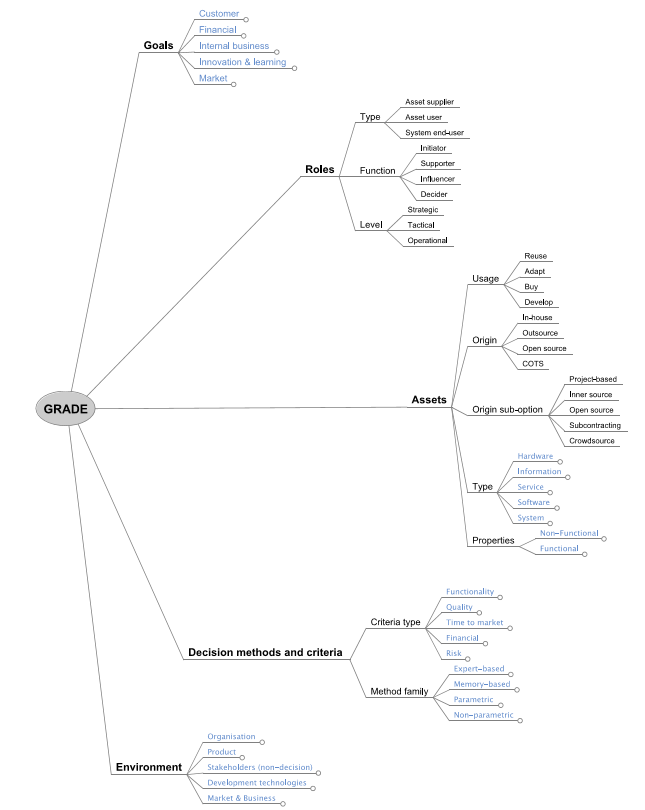
\includegraphics[width=\textwidth]{figuras/fig-grade-taxonomy} 
%	\caption{An overview of the Grade Taxonomy~\cite{papatheocharous2018thegrade}.}
%	\label{fig-grade-taxonomy}
%\end{figure}

The GRADE taxonomy is built for a specific decision-making sub-domain, its elements are specializations of Basic Decision Theory (BDT)~\cite{decision-theory} concepts, i.e. acts, events, outcomes, and payoffs. Therefore, in order to provide a precise semantic account of the concepts composing the GRADE taxonomy, it is essential to understand well the BDT elements.

In BDT, acts are the actions considered by the agent. For instance, when leaving, the agent can ``carry the umbrella'' or ``not carry the umbrella''. Events are occurrences beyond the control of the agent, e.g., the possibility of rain. Outcomes are the result of the occurrence of acts and events. For example, ``getting wet or not'' and ``carrying or not the weight of the umbrella''. Payoffs are judgments of value that the decision maker makes for each outcome. For example, how much is it worth being free from the bother of carrying an umbrella in face of the possibility of rain?


\subsection{Decision-making Ontology}
\label{subsec-decision-making}

The Decision-making Ontology (DMO)~\cite{guizzardi2018aligning} is a core ontology composed of the basic concepts underlying the decision-making process. DMO is grounded on the UFO foundational ontology~\cite{guizzardi:phdthesis05}, thus reusing and specializing UFO concepts. Figure~\ref{fig-decision-making-ontology} presents DMO's conceptual model.

\begin{figure}
	\centering
	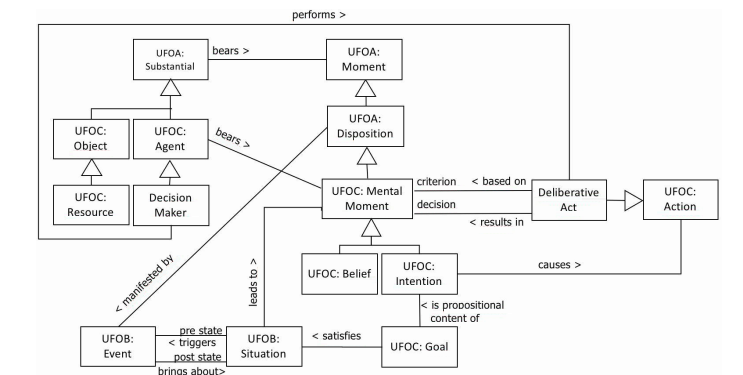
\includegraphics[width=\textwidth]{figuras/fig-decision-making-ontology} 
	\caption{The Decision-Making Ontology~\cite{guizzardi2018aligning} conceptual model.}
	\label{fig-decision-making-ontology}
\end{figure}

In DMO, a \textit{Deliberative Act} is an \textit{Action} performed by a \textit{Decision-Maker}, which is the \textit{Agent} responsible for making a \textit{Decision}. In its turn, a \textit{Decision} is a \textit{Mental Moment} (more specifically, an \textit{Intention} or a \textit{Belief}) that inheres in (being existentially dependent on) the \textit{Decision-Maker}. Additionally, the Decision-Maker may use some criteria to make a decision. A \textit{Criterion} is also a \textit{Mental Moment} of the \textit{Decision Maker}. Finally, it is important to explain that the \textit{Goal} aimed by \textit{Decision-Maker} when executing the \textit{Deliberative Act} attempts to achieve a particular \textit{Situation} of the world. In other words, the \textit{Decision-Maker} attempts to change the state of the world from a Situation A to a Situation B, which is compliant with his \textit{Intention}.


%%% Section start %%%
\section{Ontological Analysis}
\label{sec-ontology}
According to Guarino ~\cite{ontological-analysis}, “Ontological analysis can be defined as the process of eliciting and discovering relevant distinctions and relationships bound to the very nature of the entities involved in a certain domain, for the practical purpose of disambiguating terms having different interpretations in different contexts.” A good practice here is using a reference ontology, i.e. an explicit and formal representation of a conceptualization of that domain ~\cite{guizzardi:phdthesis05}. Performing an ontological analysis with the use of a reference ontology means interpreting the analyzed domain in terms of the concepts defined in this ontology. This process is aimed at grounding the semantics of the concepts of the domain of interest using the reference ontology. For that, it is paramount to choose a reference ontology of high quality, as this ontology is assumed to be a complete and semantically sound representation of the domain of interest.

In this work, we apply the Decision-Making Ontology (DMO), a well-founded ontology, as the ontological analysis's reference ontology.  Being well-founded means that the concepts of DMO are defined in terms of a foundational ontology (in this case, UFO). As a result, the concepts of DMO have not been defined from scratch. Instead, they have been grounded in the concepts of the foundational ontology, also importing their formal semantics and ontological commitments. This is aimed at making DMO a semantically sound ontology.

In this section, we analyze the definitions of the elements of the GRADE taxonomy and Basic Decision Theory (BDT), that were formally presented in Section~\ref{sec-background}, and evaluate them with the definitions from DMO. Further, we also propose the creation of new concepts or the generalization of existing ones, in order to better explain and represent certain parts of the decision-making domain. 

As we have shown in Section~\ref{sec-background}, the GRADE taxonomy consists of five top-level elements: Goals, Roles, Assets, Decision Methods \& Criteria, and Environment. In turn, each of these elements are further refined in lower-level elements that are intended to represent different perspectives of the top-level ones. However, since the lower-level elements are related to perspectives that are domain-dependent, we will focus only on the top-level ones, which are domain independent, and thus covered by our chosen reference ontology.

In the following subsections, we will use different colors to represent concepts of distinct sources. UFO and DMO concepts are colored in yellow. GRADE concepts are orange. BDT concepts are colored in blue. Finally, new concepts, are presented in green. This decision was made with the goal to clarify where each reused concept fits in our ontology and the new concepts created by it.

%Figure~\ref{fig-colors} presents the types of concepts and their colors.
%\begin{figure}
%	\centering
%	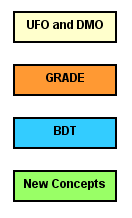
\includegraphics{figuras/fig-colors} 
%	\caption{Presents the types of concepts and the colors that were used.}
%	\label{fig-colors}
%\end{figure}

\subsection{Decision Method and Criteria}

As can be seen in Figure~\ref{fig-decision-making-ontology}, DMO represents both \textit{Criteria} and \textit{Decision} as UML roles, directly connecting \textit{Mental Moment} to Deliberative Act. Here, we prefer to use concepts to represent \textit{Criteria} and \textit{Decision}, because it makes it easier to represent the relation between these concepts and other concepts. 

Although DMO represents the criteria and the result of a decision making, it does not mention the method used in this process. Since this is a concept in the GRADE taxonomy, we suggest the inclusion of the \textit{Decision Method} concept. According to UFO, a decision method can be seen as a \textit{Complex Action Universal}, i.e. a process that will be followed by someone when taking a decision. We define it as a Universal (i.e. type) rather than an Particular (i.e. instance), because the method defines in the type level, the set of activities to be followed. In this sense, the \textit{Deliberative Act} may be seen as a instance of the \textit{Decision Method}.

Figure~\ref{fig-ontology-criteria-decision-method2} presents the new concepts that are being proposed.
\begin{figure}
	\centering
	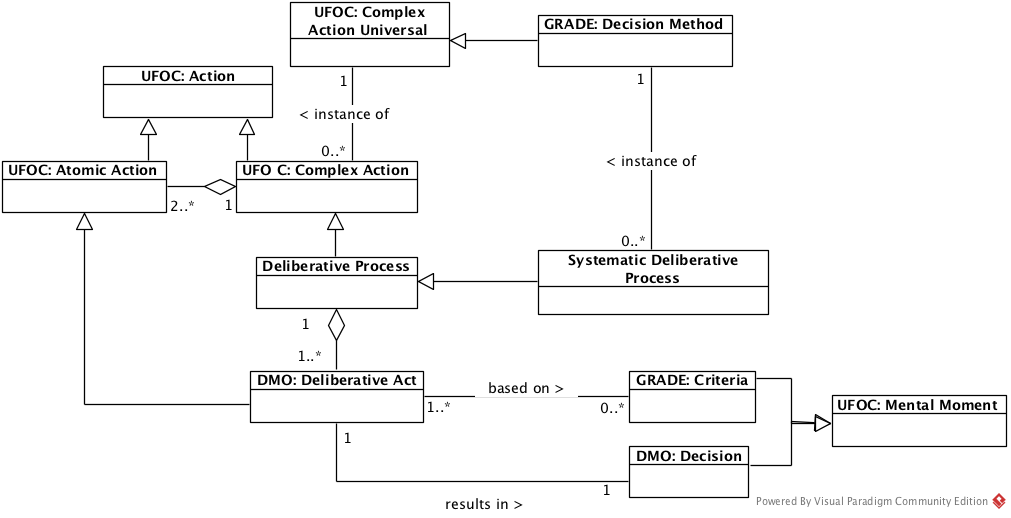
\includegraphics[width=\textwidth]{figuras/deliberative-process}
	\caption{Fragment of the Ontological Analysis that represents the \textit{Decision Method} and the \textit{Criteria}}
	\label{fig-ontology-criteria-decision-method2}
\end{figure}


\subsection{Roles}

The only role (in the sense of UFO-C:Agent) considered in DMO is the \textit{Decision Maker}, GRADE, on the other hand, considers other roles for people which are involved in the decision-making. These Decision Stakeholders are \textit{Agents} (persons, groups or even organizations) who, in some way, influence decision-making process. We will consider that this "influence" is to give a \textit{Criteria} that will base the \textit{Decision Method}. Therefore, every \textit{Criteria} is given by a \textit{Decision Stakeholder}, which in turn assigns a value to that \textit{Criteria}. It means that the \textit{Decision Stakeholder} performs an \textit{Evaluation} using the criteria. In its turn, the \textit{Decision Maker} is, a specific type of \textit{Decision Stakeholder} that makes the final decision (and that is considered responsible by it). For example, during the World War II, Winston Churchill said: "\textit{Gentlemen, what I expect from you is that after a reasonable amount of time and discussion, everyone in this room will agree with me}". In this example, Churchill made clear that although there were many \textit{Decision Stakeholders} in the room, he is the \textit{Decision Maker}, responsible for the \textit{Deliberative Act}. Finally, it is important to mention that each \textit{Criteria} can be evaluated for different value perspectives.

Figure~\ref{fig-ontology-decision-stakeholder} presents the relations between the \textit{Decision Stakeholder} and the \textit{Criteria}.

\begin{figure}
	\centering
	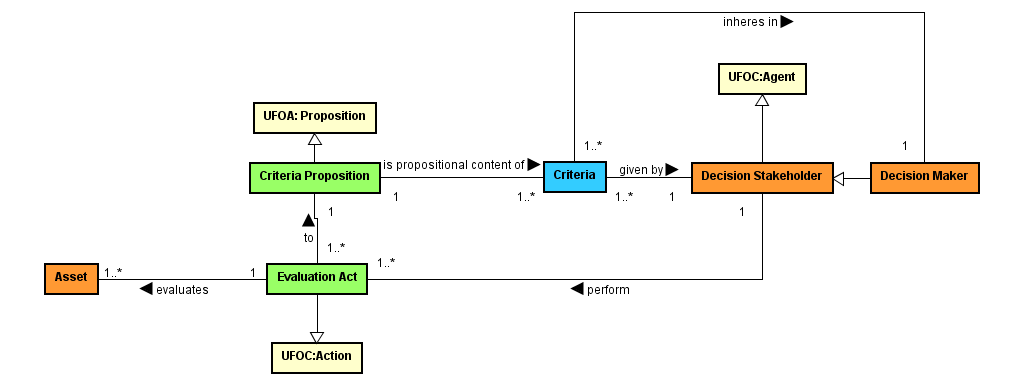
\includegraphics[width=\textwidth]{figuras/fig-ontology-decision-stakeholder} 
	\caption{Fragment of the Ontological Analysis that presents the concept of \textit{Decision Stakeholder}.}
	\label{fig-ontology-decision-stakeholder}
\end{figure}


\subsection{Assets}

The GRADE taxonomy is not clear about the definition of \textit{Asset}, however, it gives us some examples of assets (hardware, software or systems composed by hardware and software) that allow us to infer that \textit{Asset} is a type of \textit{Object}.   Moreover, in an GRADE application , \textit{Assets} can be considered architectural options in the decision making, thus, comparable to Acts in TBD, with the difference that in TBD the options are more generic since it is in an domain-independent decision-making process. In this work we opted for use the word "Option" instead of "Acts" to name the concept that represents the options considered in a decision making. So \textit{Option} is an \textit{Individual} (can be a \textit{Endurant} like a software or an \textit{Perdurant} like an Action to be performed by the Decision Maker) considered by the \textit{Decision Maker} as an possible result in a \textit{Deliberative Act}.
It should also be noted that being an \textit{Asset} by itself is not sufficient cause for this \textit{Asset} to be in a decision-making context. It will only be in this context if it is indicated as an option in a decision-making process by a \textit{Decision Stakeholder}. Moreover, this \textit{Option} is indicated by an \textit{Action} defined as \textit{Option Indication}, which is performed by a \textit{Decision Stakeholder}.

Figure~\ref{fig-ontology-assets} presents a fragment of our ontology that represents the ontological nature of \textit{Assets}.


\begin{figure}
	\centering
	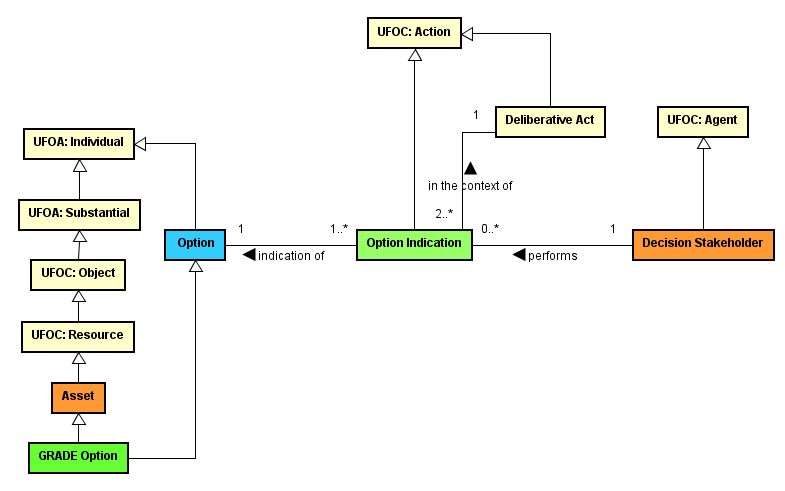
\includegraphics[width=\textwidth]{figuras/fig-ontology-assets} 
	\caption{Ontology fragment that contemplates concepts of \textit{Asset} and \textit{Option}.}
	\label{fig-ontology-assets}
\end{figure}

An \textit{Option} is created in an indication (\textit{Option Indication}) by a \textit{Stakeholder}. Each indication creates an \textit{Expectation} that, if chosen, it will result in a possible situation. It is similar to "Outcome" in BDT. This \textit{Expectation} will influence the decision making thus it is a type of \textit{Criteria}.

Each \textit{Criteria} has its propositional content evaluated (\textit{Evaluation}) by the \textit{Decision Stakeholder} who indicates it. This \textit{Evaluation} is similar to "Payoff" in BDT.

Figure~\ref{fig-evaluate-indication} presents a fragment of our ontology that represents the evaluation of \textit{Option}.


\begin{figure}
	\centering
	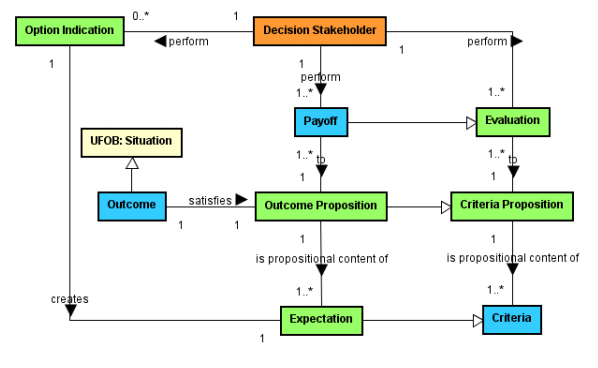
\includegraphics[width=\textwidth]{figuras/fig-evaluate-indication} 
	\caption{Ontology fragment that contemplates concepts of \textit{Option} and \textit{Evaluation}.}
	\label{fig-evaluate-indication}
\end{figure}

\subsection{Goals}

It is clear that \textit{Goals}, \textit{Intentions} and even \textit{Beliefs} of a \textit{Decision Maker} can influence his Decisions. Because of that, we have a type of Criteria that is associated with that goal. The concepts of \textit{Goal} and \textit{Intention} of UFO-C can be associated with the concept of Goal in GRADE. However, a \textit{Goal} in UFO-C extrapolates the decision context, that is, not every instance of \textit{Goal} is associated with a instance of \textit{Deliberative Act}. This association occurs through a particular type of \textit{Intention}. Therefore, we propose the creation of two new concepts: \textit{Decision Goal} and \textit{Decision Intention} with the following definitions:
Decision Intention: This is a type of \textit{Criteria} and \textit{Intention} that represents the purpose of the \textit{Decision Maker}.
Decision Goal: It is a \textit{Goal} that is the propositional content of a \textit{Decision Intention}.

Figure~\ref{fig-ontology-goals} presents a fragment of our ontology that represents a \textit{Goal} and its relations.

\begin{figure}
	\centering
	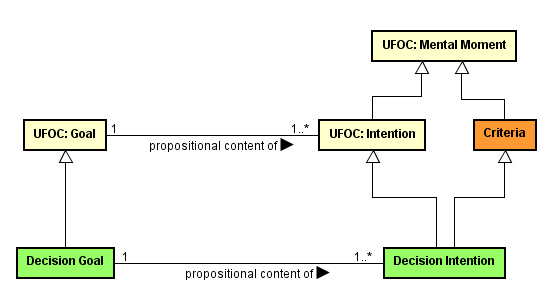
\includegraphics[width=\textwidth]{figuras/fig-ontology-goals} 
	\caption{Ontology fragment that contemplates the concept of \textit{Goal}.}
	\label{fig-ontology-goals}
\end{figure}

Each \textit{Criteria} has your proposition content evaluated by the \textit{Decision Stakeholder} who indicates it. The GRADE indicates a list of value perspectives under which the Goals can be evaluated. In this work, we represent these perspectives as generalizations of the new concept \textit{Goal Value Perspective}. In other words, \textit{Goal Value Perspectives} are \textit{Value Perspectives} in the context of a \textit{Goal Evaluation} and a \textit{Goal Evaluation} is an \textit{Evaluation} of a \textit{Decision Goal}.

Figure~\ref{fig-goal-evaluation} presents a fragment of our ontology that represents a \textit{Goal Evaluation} and \textit{Goal Value Perspective}.

\begin{figure}
	\centering
	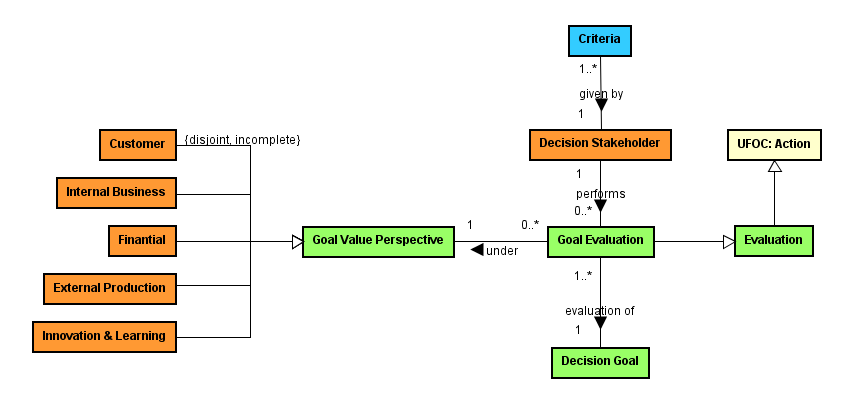
\includegraphics[width=\textwidth]{figuras/fig-goal-evaluation} 
	\caption{Ontology fragment that represents a \textit{Goal Evaluation} and its relations.}
	\label{fig-goal-evaluation}
\end{figure}


\subsection{Environment}


In GRADE, \textit{Environment} is defined as a fact that is in the context of the decision but beyond the control of \textit{Decision Maker}. In this sense, we can understand a "fact" as a portion of reality that exists in its own. This is exactly the definition of \textit{Situation} in UFO-A. In~\cite{guizzardi-et-al:er13}, Guizzardi proposes a theory where \textit{Situations}, as states of affairs, can be divided in "Factual", which are Situations that are obtained at a time point (e.g the situation where Donald Trump is president of the United States) and "Counterfactual", which never are obtained in a time point. Because of that, we propose that the concept of \textit{Environment} should be renamed to \textit{Environmental Fact} and understood as a factual \textit{Situation}, as it is defined in UFO and used in DMO. In other words, they represent a portion of the reality, prior to the \textit{Deliberative Act}. Besides that, in this work, we propose that what influences the decision are \textit{Mental Moments} (\textit{Criteria}). Therefore, we created the concepts of \textit{Environment Proposition}, which is an abstract representation of the \textit{Environment}, based on a moment of the \textit{Decision Maker}. Finally, it is important to explain that, as it is defined in UFO, after the occurrence of an \textit{Event//Action} (in this case, the \textit{Deliberative Act}) a new Situation will be brought into existence, the one that was created by the occurrence of \textit{Deliberative Act}, however this new situation cannot be considered a \textbf{post-state} \textit{Environment}, since it would violate the definition that is presented in the taxonomy.


Figure~\ref{fig-ontology-environment} presents the ontological nature of the concept \textit{Environment}.

\begin{figure}
	\centering
	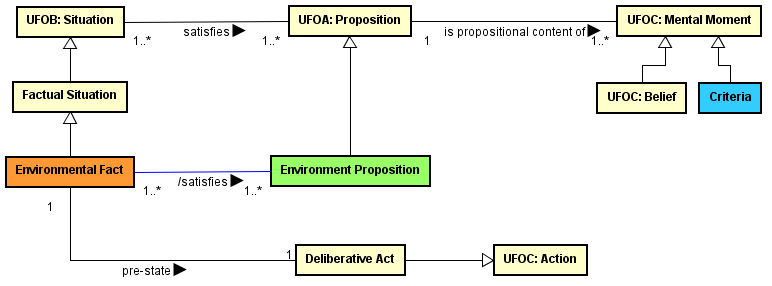
\includegraphics[width=\textwidth]{figuras/fig-ontology-environment} 
	\caption{Fragment of the Ontological Analysis that presents the concept \textit{Environment}.}
	\label{fig-ontology-environment}
\end{figure}
\section{Illustrative Example}
\label{sec-example}
%2p.(methodology configuration/architectural decisions, which can be supported by the SUPERSEDE toolsuite) for a specific project
%Discussion about the added value of using the ontology in the example

Here we use the GRADE taxonomy to configure the architecture of SUPERSEDE~\footnote{SUPERSEDE stays for SUpporting evolution and adaptation of PERsonalized Software by Exploiting
contextual Data and End-user feedback. It is an H2020 EU funded project,
http://www.supersede.eu.} to describe the activity of \textit{collaborative Requirements Prioritization} and \textit{next release planning} where user feedback is considered as one of the sources of requirements.

The analysis is based on the recognition of the different ontological elements characterizing the activity in the GRADE taxonomy. These elements should be able to describe the activity of configuring an instance of the SUPERSEDE methodology. 

~\cite{FranchRPAAGNOSS18,BusettaKMPSS17,KifetewMPSSB17_RE17demo,ameller2017replan} 
\begin{itemize}
    \item The overall \textsf{\textbf{Goal}} of the decision activity is the Collaborative Requirements Prioritization and next release planning actively exploiting user feedback. The activity is mainly for \textsf{Internal Business} in order to \textsf{Minimize time-to-market} by improving the performances of the decision makers to allow for faster decisions.
    \item The available \textsf{\textbf{Assets}} of the SUPERSEDE methodology are the feedback gathering, the feedback analyzer (to retrieve sentiment and intentions of the feedback), the collaborative decision making methods and next release components that use Genetic Algorithms and the Analytic Hierarchy Process. These assets will be \textsf{used} and possibly \textsf{adapted} to the particular organizational context. All these assets that are both \textsf{Software} and textual have an \textsf{Open Source} \textsf{Origin}. 
    \item The \textsf{\textbf{Decision method}} for the SUPERSEDE configuration is \textsf{expert-based} and collaborative and the \textsf{\textbf{criteria}} are mainly related to the minimization of the \textsf{time-to-market} and improvement of the quality of decisions
    \item The organizational \textsf{\textbf{Roles}} involved are the \textsf{asset supplier}, and the \textsf{system end-user}; they are \textsf{deciders} at the strategic, tactical and operative levels. 
    \item Finally, the \textsf{\textbf{Environment}} of the decision is the \textsf{organization} itself.
\end{itemize}

The GRADE framework is able to capture the different elements that characterize the configuration decision for a particular goal. The missing aspects are related for example to the relationships between the different elements in the taxonomy to support an operative view of the decision. An example is given by the relationships between the Decision stakeholder and the Asset one should decide on. In the extended ontology has been identified a new intermediate concept that is Evaluation Act (see Figure~\ref{fig-ontology-decision-stakeholder}). In the case of our domain, this is reified via decision making activities related to the choice of a component that consider the asset, taking into account several criteria propositions. This is the case of the evaluation to be made to introduce the SUPERSEDE activity \textit{Feedback Gathering} that has the objective of automatically acquiring and analyzing feedback or to continue processing the feedback by hand. This Evaluation Act can be executed on the bases of different criteria (such as speed in the decision, accuracy and collaboration among decision makers) and using different tools (such as decision tables or algorithms embedded in the SUPERSEDE explorer service \url{https://www.supersede.eu/downloads/supersede-method-explorer/})

%%% Section start %%%
\section{Related Work}
\label{sec-relatedwork}
%[Anna] Related work (0,7 p.)
%Using ontology for decision making?
%Ontological analysis of other decision-making methods?

Mansingh and Rao~\cite{mansingh2014enhancing} present a method for enhancing the decision making process that is based in an organizational ontology. Authors argue that the ontology can be used to provide a better understanding of the domain in which the decision is being made. A series of steps are presented for the decision-maker to follow, these steps are organized in a way to focus on the understanding of the consequences of each alternative of the decision that is being made. Authors also suggest that a potential user of the method should create an that represents the domain of the decision.  In comparison with our ontological analysis and with the decision-making ontology, the term ontology here seems to be used in a loose way, since the paper does not provide a reference model of the referred ontology. The organizational ontology that is mentioned is presented in a taxonomy of core elements of the decision-making domain, such as goals, resources, tasks and roles, however, the relations between these elements are not properly explained. 

Chai and Liu~\cite{chai2010ontology} proposed a ontology-based framework focused on group decision process, called ONTOGDSS. Authors claim that the framework the management of the group decision-making process as a whole, from the evaluation of the alternatives to the aggregation of the decision, since the embedded ontology structure provides formal description features to facilitate the decision analysis. ONTOGDSS consists in two aspects: a group decision process, which should be followed and a hierarchical structure, which is composed by four layers, where the fourth one, called \textit{Ontology based Decision-resource layer} uses semantic extraction to represent and describe the decision problems that are stored in heterogeneous databases. In other words, ONTOGDSS defines a set of meta-data to describe attributes, objectives, constraints and criteria that are part of the decision process. Furthermore, with the properties and limitations of the decision problem represented, it can be analyzed accordingly, with tools like Ontobroker.

\section{Discussion}
\label{sec-discussion}
%[Anna]Discussion (1.3 p.)
%Threat to validity?
%Implication of this work
Potential follow-ups:\\
- “Easy” and coherent extension of GRADE\\
- Use of “competency questions” for extending the ontology to the “domain dependent level\\
- Ontology validation techniques could be used to validate the guideline for decision-making

%%% Section start %%%
\section{Conclusions}
\label{sec-conclusions}

In this paper we have presented an ontological analysis of the GRADE taxonomy, originally proposed in~\cite{papatheocharous2015decision}. We believe that this work can be used as an initial discussion towards a more expressive version of The GRADE taxonomy, one that takes into consideration the ontological nature of the concepts and relations that exists between them. We argue that DMO and the work presented here are the first steps towards this goal.

As future work, we intend to dig deeper into this subject by analyzing the decision-making domain with the Ontology of Value and Risk~\cite{value-risk-2018}. We argue that Value and Risk are concepts that are intrinsically connected to the decision-making process, and should thus enrich and complement the concepts already considered in DMO.



% Acknowledgments.
%\section{Acknowledgments}
%Nemo (\url{http://nemo.inf.ufes.br}) is currently supported by Brazilian research agencies Fapes (\# 0969/2015), CNPq (\# 461777/2014-2), and by Ufes' FAP (\# 6166/2015). We would like to thank Nicola Guarino, Pedro Negri and Beatriz Franco Martins for their participation during discussions about the research contained herein.


% Bibliography.
\bibliographystyle{myunsrt}
\bibliography{Ontological-Analysis-GRADE-Taxonomy}

% The end.
\end{document}
